% Appendix A

\chapter{Esquemas de las red, Códigos y Resultados obtenidos} % Main appendix title


\label{AppendA} % For referencing this appendix elsewhere, use \ref{AppendixA}


\section{Esquemas}\label{esquemas}
\subsection{RNN simple}\label{RNNNNN}
\begin{figure}[H]
	\begin{center}
		\begin{tikzpicture}[node distance=2cm]
		\node (i1) [startstop] {Input Layer};
		\node (i2) [startstop, below of=i1] {Recurrent Layer};
		
		\node (i3) [startstop, below of=i2] {Dense Layer};
		\node (i4) [startstop, below of=i3] {Output Layer};
		\draw [arrow] (i1) -- (i2) ;
		\draw [arrow] (i2) -- (i3);
		\draw [arrow] (i3) -- (i4);
		\end{tikzpicture}
	\end{center}
	\caption{Esquema de  RNN simple \\ Fuente:  \textit{Fuente Propia}}
\end{figure}


\subsection{LSTM simple}\label{LSTMESQUEMA}
\begin{figure}[H]
	\begin{center}
		\begin{tikzpicture}[node distance=2cm]
		\node (i1) [startstop] {Input Layer};
		\node (i2) [startstop, below of=i1] {LSTM Layer};
		
		\node (i3) [startstop, below of=i2] {Dense Layer};
		\node (i4) [startstop, below of=i3] {Output Layer};
		\draw [arrow] (i1) -- (i2) ;
		\draw [arrow] (i2) -- (i3);
		\draw [arrow] (i3) -- (i4);
		\end{tikzpicture}
	\end{center}
	\caption{Esquema de LSTM simple \\ Fuente:  \textit{Fuente Propia}}
\end{figure}


\subsection{LSTM con Dropout}\label{LSTMESQUEMA1DROP}
\begin{figure}[H]
	\begin{center}
		\begin{tikzpicture}[node distance=2cm]
		\node (i1) [startstop] {Input Layer};
		\node (i2) [startstop, below of=i1] {LSTM Layer};
		\node (i3) [startstop, below of=i2] {Dropout};
		\node (i4) [startstop, below of=i3] {Dense Layer};
		\node (i5) [startstop, below of=i4] {Output Layer};
		\draw [arrow] (i1) -- (i2) ;
		\draw [arrow] (i2) -- (i3);
		\draw [arrow] (i3) -- (i4);
		\draw [arrow] (i4) -- (i5);
		\end{tikzpicture}
	\end{center}
	\caption{Esquema de LSTM con dropout \\ Fuente:  \textit{Fuente Propia}}
\end{figure}

\subsection{2 capas LSTM  con 2 Dropout}\label{2LSTMESQUEMA}
\begin{figure}[H]
	\begin{center}
		\begin{tikzpicture}[node distance=2cm]
		\node (i1) [startstop] {Input Layer};
		\node (i2) [startstop, below of=i1] {LSTM Layer};
		\node (i3) [startstop, below of=i2] {Dropout};
		\node (i4) [startstop, below of=i3] {LSTM Layer};
		\node (i5) [startstop, below of=i4] {Dropout};
		\node (i6) [startstop, below of=i5] {Dense Layer};
		\node (i7) [startstop, below of=i6] {Output Layer};
		\draw [arrow] (i1) -- (i2) ;
		\draw [arrow] (i2) -- (i3);
		\draw [arrow] (i3) -- (i4);
		\draw [arrow] (i4) -- (i5);
		\draw [arrow] (i5) -- (i6);
		\draw [arrow] (i6) -- (i7);
		\end{tikzpicture}
	\end{center}
	\caption{Esquema de 2 capas LSTM con 2 dropout \\ Fuente:  \textit{Fuente Propia}}
\end{figure}


\newpage
\section{Códigos}
\subsection{Conversión de formatos}\label{converter}
\begin{lstlisting}[language=Bash,caption=Bash para conversión de formato,captionpos=b]
# itera los archivos .ogg
for i in *.ogg;
# realiza la conversion ogg a wav usando ffmpeg
do ffmpeg -i "$i" "${i%.*}.wav"; 
done

\end{lstlisting}

\subsection{Obtención de coeficientes MFCC}\label{MFCCC}
\begin{lstlisting}[language=Python,caption=Obtención de MFCC,captionpos=b]
# cargado del audio
wave, sr = librosa.load(DIR+dir, mono=True)
# obtencion de los coeficientes
features= librosa.feature.mfcc(wave, sr,n_mfcc=20)
#padding con ceros asegurar misma dimension de salida
features=np.pad(features,((0,0),(0,160-len(features[0]))),
mode='constant',constant_values=0)

\end{lstlisting}

\subsection{One hot encoding}\label{onehot}

\begin{lstlisting}[language=Python,caption=one hot encoding,captionpos=b,xleftmargin=.05\textwidth]
from sklearn.preprocessing import OneHotEncoder
# vocabulario de clases definidas
vocabulary_words=np.array(['cero','uno','dos','tres',
'cuatro','cinco','seis','siete','ocho','nueve'])
onehot_encoder = OneHotEncoder(handle_unknown='ignore',
categories='auto')
# entrenamiento del OneHotEncoder
onehot_encoder.fit(X=vocabulary_words.reshape(-1,1))
\end{lstlisting}

\subsection{RNN}\label{RNNCODE}

\begin{lstlisting}[language=Python,caption=Modelo LSTM,captionpos=b,xleftmargin=.05\textwidth]
# establece la secuencia para empezar con el apilado de capas
model=tf.keras.Sequential()
# se apila una capa RNN simple 
model.add(tf.keras.layers.SimpleRNN(128, input_shape=(time_steps,n_inputs)))
# establece una capa densamente conectada
model.add(tf.layers.Dense(n_class, activation='softmax'))

\end{lstlisting}
\subsection{LSTM Simple}\label{LSTMCODE}
\begin{center}
	\begin{lstlisting}[language=Python,caption=Modelo LSTM,captionpos=b,xleftmargin=.05\textwidth]
	# usado para apilar las capas de la red
	model=tf.keras.Sequential()
	# apila una capa LSTM
	model.add(tf.keras.layers.LSTM(n_units,
	input_shape=(time_steps,n_inputs)))
	# establece una capa densamente conectada
	model.add(tf.layers.Dense(n_class, activation='softmax'))
	
	
	\end{lstlisting}
\end{center}
\subsection{LSTM con Dropout}\label{LSTMCODEDROP}

\begin{center}
	\begin{lstlisting}[language=Python,caption=Modelo LSTM,captionpos=b,xleftmargin=.05\textwidth]
	model=tf.keras.Sequential()
	# apila una capa LSTM
	model.add(tf.keras.layers.LSTM(n_units,
	input_shape=(time_steps,n_inputs)))
	# apila un Dropout a nuestra red para evitar overfitting
	model.add(tf.keras.layers.Dropout(0.5))
	# establece una capa densamente conectada
	model.add(tf.layers.Dense(n_class, activation='softmax'))
	
	
	\end{lstlisting}
\end{center}
\subsection{2 Capas LSTM con 2 Dropout}\label{2LSTM2DROPCODE}
\begin{center}
	\begin{lstlisting}[language=Python,caption=Modelo 2 capas LSTM y 2 dropout,captionpos=b,xleftmargin=.05\textwidth]
model=tf.keras.Sequential()
#primera capa LSTM
model.add(tf.keras.layers.LSTM(n_units, input_shape=(time_steps,n_inputs),return_sequences=True))
# aplicacion del Dropout
model.add(tf.keras.layers.Dropout(dropout))
# 2da capa LSTM
model.add(tf.keras.layers.LSTM(n_units, input_shape=(time_steps,n_inputs)))
# 2da aplicacion del Dropout
model.add(tf.keras.layers.Dropout(dropout))
model.add(tf.layers.Dense(n_class, activation='softmax'))
	\end{lstlisting}
\end{center}
\subsection{Configuración del modelo}\label{configmodel}
\begin{lstlisting}[language=Python,caption=Parámetros para el entrenamiento del modelo,captionpos=b,xleftmargin=.05\textwidth]
# configura el entrenamiento del modelo
model.compile(loss='categorical_crossentropy',
optimizer='adam',metrics=['accuracy'])
\end{lstlisting}
\subsection{Entrenamiento del modelo}\label{trainingmodel}
\begin{lstlisting}[language=Python,caption=Entrenamiento del modelo,captionpos=b,xleftmargin=.05\textwidth]
# entrenamiento del modelo pasando train and test set
history=model.fit(trainX,trainY,batch_size=batch_size,
epochs=n_epochs,validation_data=[testX,testY])
\end{lstlisting}

\section{Pruebas con RNN, LSTM con MFCC}
\subsection{Resultados de precisión de entrenamiento}\label{precision}
\subsubsection{64 estados ocultos}\label{64stateprec}
\begin{figure}[H]
	\centering
	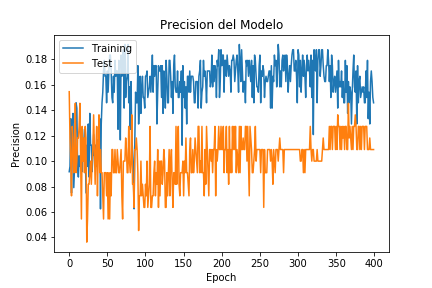
\includegraphics[width=0.7\textwidth]{Figures/rnn_64_prec}
	\caption{Precisión de RNN para 64 estados ocultos\\ Fuente: {\textit{Fuente Propia}}}
	\label{RNNSIMPLE64}
\end{figure} 
\begin{figure}[H]
	\centering
	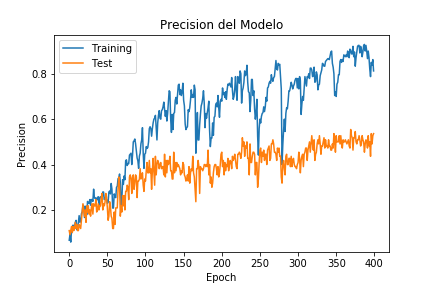
\includegraphics[width=0.7\linewidth]{Figures/lstm13_64_prec}
	\caption{Precisión de LSTM simple para 64 estados ocultos\\ Fuente: {\textit{Fuente Propia}}}
	\label{fig:lstm1364prec}
\end{figure}

\begin{figure}[H]
	\centering
	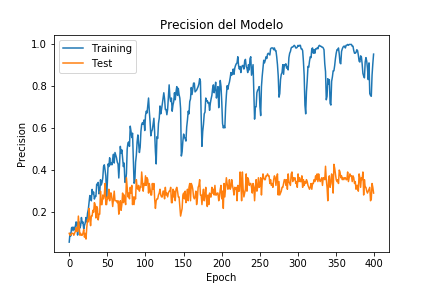
\includegraphics[width=0.7\linewidth]{Figures/lstm_64_05_prec}
	\caption{Precisión LSTM con dropout 0.5 para 64 estados ocultos\\ Fuente: {\textit{Fuente Propia}}}
	\label{fig:lstm6405prec}
\end{figure}
\begin{figure}[H]
	\centering
	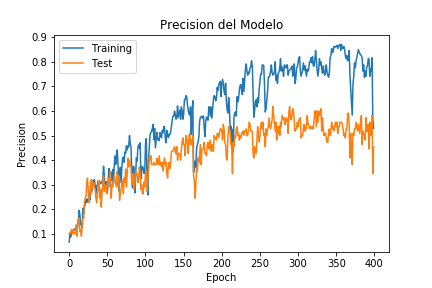
\includegraphics[width=0.7\linewidth]{Figures/lstm_64_08_prec}
	\caption{Precisión LSTM con dropout 0.8 para 64 estados ocultos\\ Fuente: {\textit{Fuente Propia}}}
	\label{fig:lstm6408prec}
\end{figure}

\subsubsection{128 estados ocultos}\label{128stateprec}
\begin{figure}[H]
\centering
	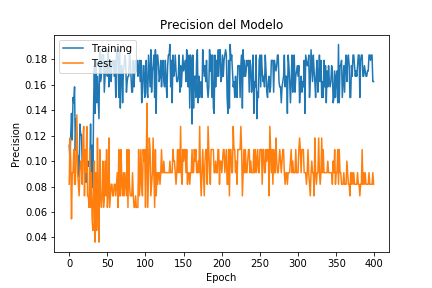
\includegraphics[width=0.7\textwidth]{Figures/rnn_prec_400_13mfcc}
	\caption{Precisión de RNN para 128 estados ocultos\\ Fuente: {\textit{Fuente Propia}}}
	\label{RNNSIMPLE}
\end{figure} 

\begin{figure}[H]
	\centering
	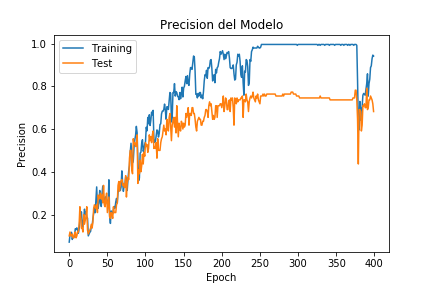
\includegraphics[width=0.7\textwidth]{Figures/lstm_400_prec_13mfcc}
	\caption{Precisión de LSTM simple para 128 estados ocultos\\ Fuente: {\textit{Fuente Propia}}}
	\label{LSTMsimpel}
\end{figure} 

\begin{figure}[H]
	\centering
	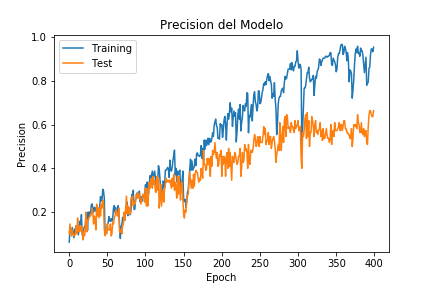
\includegraphics[width=0.7\textwidth]{Figures/lstm_400drop05_prec_13mfcc}
	\caption{Precisión de LSTM dropout 0.5 para 128 estados ocultos\\ Fuente: {\textit{Fuente Propia}}}
	\label{LSTMdropout5}
\end{figure} 


\begin{figure}[H]
	\centering
	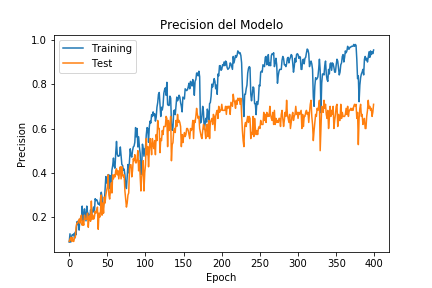
\includegraphics[width=0.7\textwidth]{Figures/lstm_400drop08_prec_13mfcc}
	\caption{Precisión de LSTM dropout 0.8 para 128 estados ocultos\\ Fuente: {\textit{Fuente Propia}}}
	\label{LSTMdropout8}
\end{figure} 
\newpage
\subsubsection{256 estados ocultos}\label{256stateprec}
\begin{figure}[H]
	\centering
	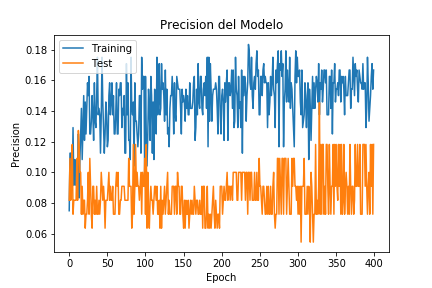
\includegraphics[width=0.7\linewidth]{Figures/rnn_256_prec}
	\caption{Precisión de RNN para 256 estados ocultos\\ Fuente: {\textit{Fuente Propia}}}
	\label{fig:rnn256prec}
	\centering
	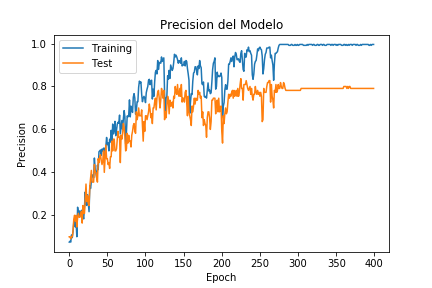
\includegraphics[width=0.7\linewidth]{Figures/lstm_256_prec13}
	\caption{Precisión LSTM simple para 256 estados ocultos\\ Fuente: {\textit{Fuente Propia}}}
	\label{fig:lstm256prec13}
\end{figure}
\begin{figure}[H]
	\centering
	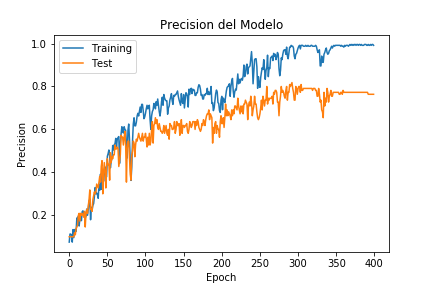
\includegraphics[width=0.7\linewidth]{Figures/lstm5_256_13prec}
	\caption{Precisión LSTM con dropout 0.5 para 256 estados ocultos\\ Fuente: {\textit{Fuente Propia}}}
	\label{fig:lstm525613prec}
	\centering
	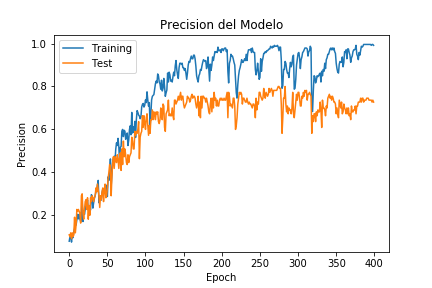
\includegraphics[width=0.7\linewidth]{Figures/lst_256_13prec}
	\caption{Precisión LSTM con dropout 0.8 para 256 estados ocultos\\ Fuente: {\textit{Fuente Propia}}}
	\label{fig:lst25613prec}
\end{figure}
\newpage

\subsection{Resultados de función de perdida}

\subsubsection{64 Estados ocultos}\label{64statecost}
\begin{figure}[H]
	\centering
	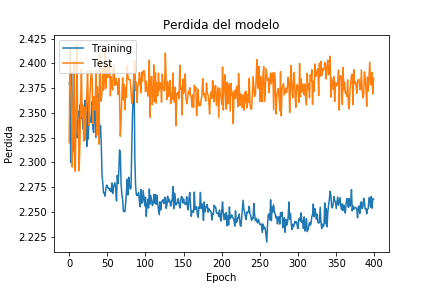
\includegraphics[width=0.7\linewidth]{Figures/rnn_64_cost}
	\caption{Perdida LSTM para 64 estados ocultos\\ Fuente: {\textit{Fuente Propia}}}
	\label{fig:rnn64cost}

	\centering
	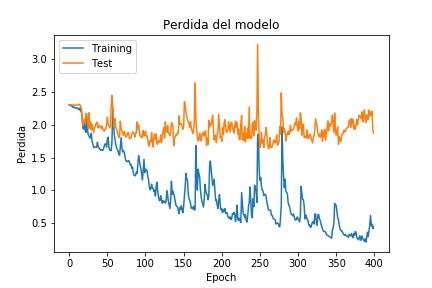
\includegraphics[width=0.7\linewidth]{Figures/lstm13_64_cost}
	\caption{Perdida LSTM  para 64 estados ocultos \\ Fuente: {\textit{Fuente Propia}}}
	\label{fig:lstm1364cost}
\end{figure}

\begin{figure}[H]
	\centering
	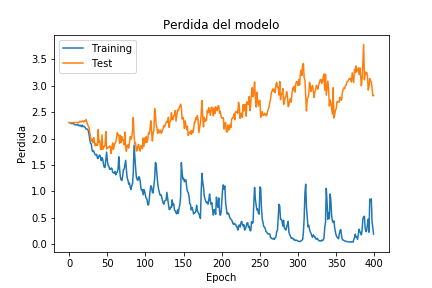
\includegraphics[width=0.7\linewidth]{Figures/lstm_64_05_cost}
	\caption{Perdida LSTM con dropout 0.5 para 64 estados ocultos\\ Fuente: {\textit{Fuente Propia}}}
	\label{fig:lstm6405cost}
	\centering
	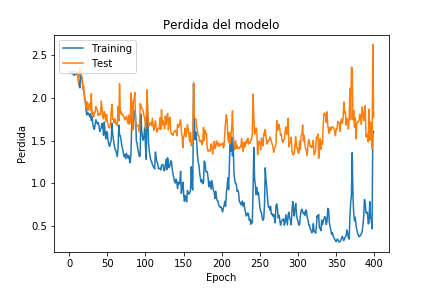
\includegraphics[width=0.7\linewidth]{Figures/lstm_64_08_cost}
	\caption{Perdida LSTM con dropout 0.8 para 64 estados ocultos\\ Fuente: {\textit{Fuente Propia}}}
	\label{fig:lstm6408cost}
\end{figure}


\subsubsection{128 estados ocultos}\label{128statecost}
\begin{figure}[H]
	\centering
	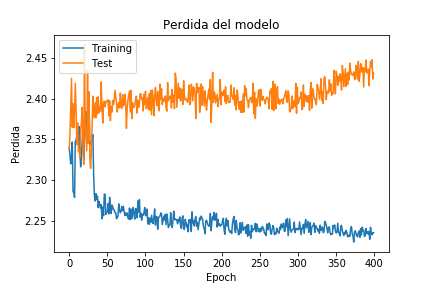
\includegraphics[width=0.7\textwidth]{Figures/rnn_cost_400_13mfcc}
	\caption{Perdida de RNN para 128 estados ocultos\\ Fuente: {\textit{Fuente Propia}}}
	\label{RNNSIMPLEcost}
\end{figure} 


\begin{figure}[H]
	\centering
	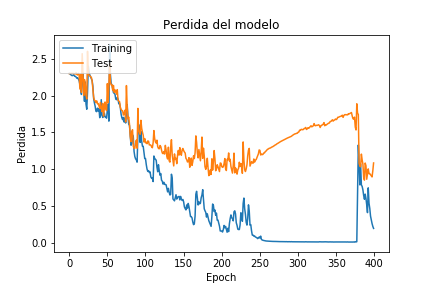
\includegraphics[width=0.7\textwidth]{Figures/lstm_400_cost_13mfcc}
	\caption{Perdida de LSTM para 128 estados ocultos\\ Fuente: {\textit{Fuente Propia}}}
	\label{LSTMsimplecost}
\end{figure} 

\begin{figure}[H]
	\centering
	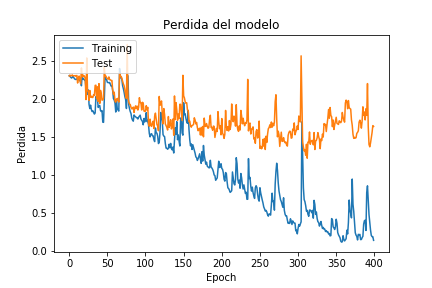
\includegraphics[width=0.7\textwidth]{Figures/lstm_400drop05_cost_13mfcc}
	\caption{Perdida de LSTM dropout 0.5 para 128 estados ocultos\\ Fuente: {\textit{Fuente Propia}}}
	\label{LSTMdropout5cost}
\end{figure} 


\begin{figure}[H]
	\centering
	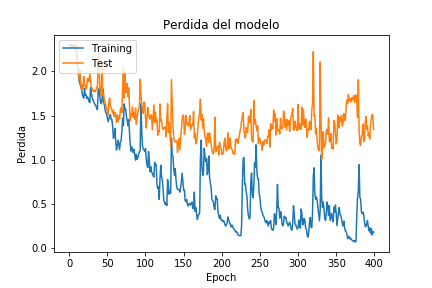
\includegraphics[width=0.7\textwidth]{Figures/lstm_400drop08_cost_13mfcc}
	\caption{Perdida de LSTM dropout 0.8 para 128 estados ocultos\\ Fuente: {\textit{Fuente Propia}}}
	\label{LSTMdropout8cost}
\end{figure} 

\subsubsection{256 estados ocultos}\label{256statecost}
\begin{figure}[H]
	\centering
	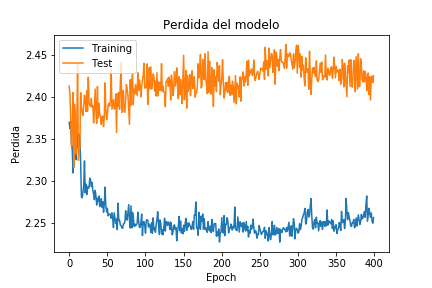
\includegraphics[width=0.7\linewidth]{Figures/rnn_256_cost}
	\caption{Perdida de RNN para 256 estados ocultos\\ Fuente: {\textit{Fuente Propia}}}
	\label{fig:rnn256cost}

	\centering
	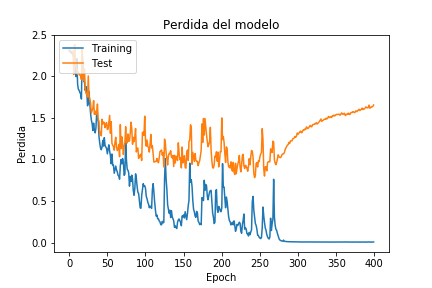
\includegraphics[width=0.7\linewidth]{Figures/lstm_256_cost13}
	\caption{Perdida de LSTM para 256 estados ocultos\\ Fuente: {\textit{Fuente Propia}}}
	\label{fig:lstm256cost13}
\end{figure}

\begin{figure}[H]
	\centering
	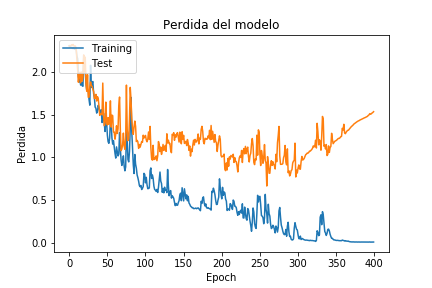
\includegraphics[width=0.7\linewidth]{Figures/lstm5_256_13cost}
	\caption{Perdida de LSTM con Dropout 0.5 para 256 estados ocultos\\ Fuente: {\textit{Fuente Propia}}}
	\label{fig:lstm525613cost}

	\centering
	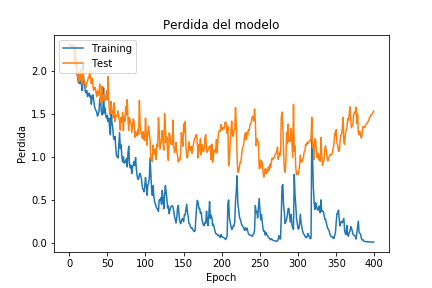
\includegraphics[width=0.7\linewidth]{Figures/lstm_256_13cost}
	\caption{Perdida de LSTM con Dropout 0.8 para 256 estados ocultos\\ Fuente: {\textit{Fuente Propia}}}
	\label{fig:lstm25613cost}
\end{figure}

\newpage

\section{Propuesta de modelo para reconocimiento de voz}\label{modelo}

\subsection{Precisión}\label{precision_modelo}

\begin{figure}[H]
	\centering
	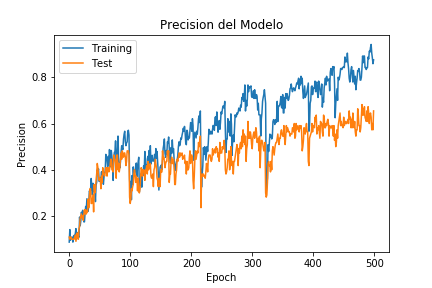
\includegraphics[width=0.7\linewidth]{Figures/MODEL_prec}
	\caption{Precisón de modelo con 2 LSTM y 2 Dropout 0.6}
	\label{fig:modelprec}
\end{figure}

\subsection{Error}\label{erro_modelo}

\begin{figure}[H]
	\centering
	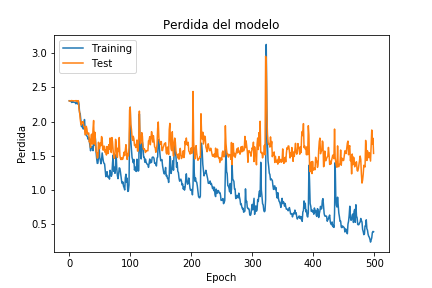
\includegraphics[width=0.7\linewidth]{Figures/MODEL_cost}
	\caption{Error de modelo con 2 LSTM y 2 Dropout 0.6}
	\label{fig:modelcost}
\end{figure}